\documentclass[twoside]{article}
\usepackage{graphicx}
\usepackage{amsmath}
\usepackage[colorlinks=true,allcolors=blue]{hyperref}
\usepackage{url}
\usepackage[top=.9in, bottom=.9in, left=1.4in, right=0.9in,a4paper]{geometry}


\begin{document}
\title{\textbf{GT4IReval: An R package to Measure the Reliability of an Information Retrieval\\Test Collection with Generalizability Theory\\{\Large Version 1.0}}}
\author{Juli\'an Urbano\\Universitat Pompeu Fabra\\\texttt{urbano.julian@gmail.com}}
\maketitle

\begin{abstract}
\noindent\texttt{GT4IReval}\footnote{For the latest version of the package and this document, please visit \url{http://julian-urbano.info}.} is a package for the statistical software \texttt{R} to measure the reliability of an Information Retrieval test collection. It allows users to estimate reliability using Generalizability Theory and map those estimates onto well-known indicators such as Kendall $\tau$ correlation or sensitivity. For background information and details, the reader is referred to \cite{Urbano2013:measurement}.
\end{abstract}

\section{Loading \texttt{GT4IReval} and Data}

The \texttt{GT4IReval} package can be loaded into \texttt{R} simply by copy-pasting the code found inside the \texttt{gt4ireval-1.0.R} file directly into the command prompt. Alternatively, it can be loaded using the \texttt{source} function with a local copy of the file:
{\small\begin{verbatim}
> source("path/to/file/gt4ireval-1.0.R")
\end{verbatim}}
\noindent or loading the latest version online from the repository\footnote{\url{https://github.com/julian-urbano/GT4IREval}}:
{\small\begin{verbatim}
> source("https://github.com/julian-urbano/GT4IREval/raw/master/gt4ireval.R")
\end{verbatim}}

\texttt{GT4IReval} needs initial evaluation data to run a G-study and the corresponding D-study. These data need to be in a standard \texttt{data.frame}, where columns correspond to systems and rows correspond to queries. For this manual, let us use data from the TREC-3 Ad Hoc track\footnote{For general information on how to read data in \texttt{R}, the reader is referred to the \textsl{R Data Import/Export} manual, accessible from \url{http://cran.r-project.org/manuals.html}.}.

{\small\begin{verbatim}
> ah3 <- read.table("adhoc3.txt")
> head(ah3)
    sys1   sys2   sys3   sys4   sys5   sys6   sys7 ...
1 0.2830 0.5163 0.4810 0.5737 0.5184 0.4945 0.5013 ...
2 0.0168 0.5442 0.3987 0.2964 0.6115 0.2354 0.1689 ...
3 0.0746 0.2769 0.3002 0.2459 0.3803 0.0738 0.0182 ...
4 0.1828 0.6622 0.6164 0.4291 0.6556 0.3529 0.3331 ...
5 0.0181 0.3670 0.3762 0.1095 0.2465 0.1027 0.0303 ...
6 0.0019 0.6752 0.6435 0.1294 0.5291 0.2087 0.2191 ...
\end{verbatim}}

If your data is transposed (i.e. columns correspond to queries and rows correspond to systems), you can get the correct format with the \texttt{t} function.

{\small\begin{verbatim}
> ah3 <- t(ah3)
\end{verbatim}}

\section{G-Study}

To run a G-study with the initial data we have, we simply call the \texttt{g.study} function.

{\small\begin{verbatim}
> g.study(ah3)

Summary of G-Study

                 Systems     Queries Interaction
             ----------- ----------- -----------
Variance       0.0071668    0.022642     0.01092
Variance(%)       17.596      55.593      26.811
---
Mean Sq.         0.36926     0.91661     0.01092
Sample size           40          50        2000
\end{verbatim}}

Additionally, we can tell the function to ignore the systems with lowest average effectiveness scores by setting the \texttt{drop} parameter. For instance, we can ignore the bottom 25\% of systems.

{\small\begin{verbatim}
> ah3.g <- g.study(ah3, drop = 0.25)
> ah3.g

Summary of G-Study

                 Systems     Queries Interaction
             ----------- ----------- -----------
Variance       0.0028117    0.028093    0.010152
Variance(%)       6.8482      68.425      24.727
---
Mean Sq.         0.15074     0.85296    0.010152
Sample size           30          50        1500
\end{verbatim}}

The summary shows the estimated variance components: variance due to the system effect $\hat\sigma_s^2=0.0028117$, due to the query effect $\hat\sigma_q^2=0.028093$, and due to the system-query interaction effect $\hat\sigma_e^2=0.010152$.
The second row shows the same values but as a fraction of the total variance. The third row shows the estimated Mean Squares for each component, and finally the sample size in each case. In our example, we have 30 systems and 50 queries as initial data.

\section{D-Study}

The results from the G-study above can now be used to run a D-study. First, let us estimate the stability of the current collection with 50 queries.

{\small\begin{verbatim}
> d.study(ah3.g)

Summary of D-Study

Call:
    queries = 50 
  stability = 0.95 
      alpha = 0.025 

Stability:
                                           Erho2                                   Phi
             -----------------------------------   -----------------------------------
     Queries    Expected       Lower       Upper      Expected       Lower       Upper
 ----------- ----------- ----------- -----------   ----------- ----------- -----------
          50     0.93265     0.89311     0.96287       0.78613     0.66141     0.88039 

Required number of queries:
                                           Erho2                                   Phi
             -----------------------------------   -----------------------------------
   Stability    Expected       Lower       Upper      Expected       Lower       Upper
 ----------- ----------- ----------- -----------   ----------- ----------- -----------
        0.95          69          37         114           259         130         487
\end{verbatim}}

The summary first shows how the \texttt{d.study} function was called. In particular, it tells us that the target number of queries is $n_q'=50$ (set by default from the G-study initial data), the target stability is $\pi=0.95$ (set by default), and the confidence level is $\alpha=0.025$ (set by default).
Next are the estimated stability scores; the relative stability with 50 queries is $\text{E}\hat\rho^2=0.93265$ with a 95\% confidence interval of $[0.89311, 0.96287]$, and the absolute stability is $\hat\Phi=0.78613$ with a 95\% confidence interval of $[0.66141, 0.88039]$.
Regarding the required number of queries to reach the target stability, the estimate is $\hat{n}_q'=69$ with a 95\% confidence interval of $[37, 114]$ to reach $\text{E}\rho^2=\pi$, and $\hat{n}_q'=259$ with a 95\% confidence interval of $[130, 487]$ to reach $\Phi=\pi$.

The \texttt{d.study} function can be called with multiple values for $n_q'$, $\pi$ and $\alpha$ to study trends. For instance, we can indicate several query set sizes by setting the \texttt{queries} parameter.

{\small\begin{verbatim}
> d.study(ah3.g, queries = seq(20,200,20))

Summary of D-Study

Call:
    queries = 20 40 60 80 100 120 140 160 180 200 
  stability = 0.95 
      alpha = 0.025 

Stability:
                                           Erho2                                   Phi
             -----------------------------------   -----------------------------------
     Queries    Expected       Lower       Upper      Expected       Lower       Upper
 ----------- ----------- ----------- -----------   ----------- ----------- -----------
          20     0.84707     0.76971     0.91208        0.5952     0.43864     0.74647 
          40     0.91721     0.86987     0.95402       0.74624      0.6098     0.85483 
          60     0.94324     0.90931     0.96887       0.81519     0.70097      0.8983 
          80     0.95682     0.93041     0.97647       0.85468     0.75761     0.92174 
         100     0.96515     0.94354     0.98109       0.88026     0.79621     0.93639 
         120     0.97079      0.9525     0.98419       0.89819      0.8242     0.94643 
         140     0.97486     0.95901     0.98642       0.91144     0.84543     0.95373 
         160     0.97793     0.96395     0.98809       0.92165     0.86209     0.95927 
         180     0.98033     0.96783      0.9894       0.92974      0.8755     0.96363 
         200     0.98227     0.97095     0.99045       0.93632     0.88654     0.96715 

Required number of queries:
                                           Erho2                                   Phi
             -----------------------------------   -----------------------------------
   Stability    Expected       Lower       Upper      Expected       Lower       Upper
 ----------- ----------- ----------- -----------   ----------- ----------- -----------
        0.95          69          37         114           259         130         487
\end{verbatim}}

The output above shows the estimated stability scores, with confidence intervals, for various query set sizes. For example, we have $\text{E}\hat\rho^2=0.96515$ with 100 queries, and $\hat\Phi\in[0.88654, 0.96715]$ with 95\% confidence when having 200 queries.
Similarly, we may indicate several target stability scores by setting the \texttt{stability} parameter.

{\small\begin{verbatim}
> d.study(ah3.g, stability = c(0.8, 0.85, 0.9, 0.95, 0.97, 0.99))

Summary of D-Study

Call:
    queries = 50 
  stability = 0.8 0.85 0.9 0.95 0.97 0.99 
      alpha = 0.025 

Stability:
                                           Erho2                                   Phi
             -----------------------------------   -----------------------------------
     Queries    Expected       Lower       Upper      Expected       Lower       Upper
 ----------- ----------- ----------- -----------   ----------- ----------- -----------
          50     0.93265     0.89311     0.96287       0.78613     0.66141     0.88039 

Required number of queries:
                                           Erho2                                   Phi
             -----------------------------------   -----------------------------------
   Stability    Expected       Lower       Upper      Expected       Lower       Upper
 ----------- ----------- ----------- -----------   ----------- ----------- -----------
         0.8          15           8          24            55          28         103 
        0.85          21          11          34            78          39         146 
         0.9          33          18          54           123          62         231 
        0.95          69          37         114           259         130         487 
        0.97         117          63         194           440         220         828 
        0.99         358         191         593          1347         673        2534
\end{verbatim}}

The output above shows that the estimated number of queries to reach $\text{E}\rho^2=0.97$ is 117, while 123 are required to reach $\Phi=0.9$.
Finally, we can also indicate several confidence levels for the computation of confidence intervals by setting the \texttt{alpha} parameter\footnote{Recall that $100(1-2\alpha)\%$ intervals are computed, so for an 80\% confidence interval we set $\alpha=0.1$.}.

\begin{figure}[b]%
\centering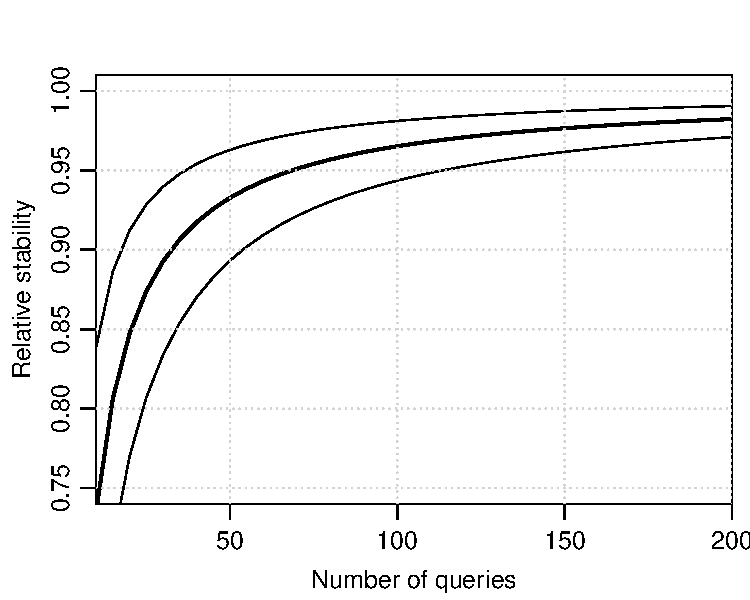
\includegraphics[scale=0.5]{plot.pdf}~~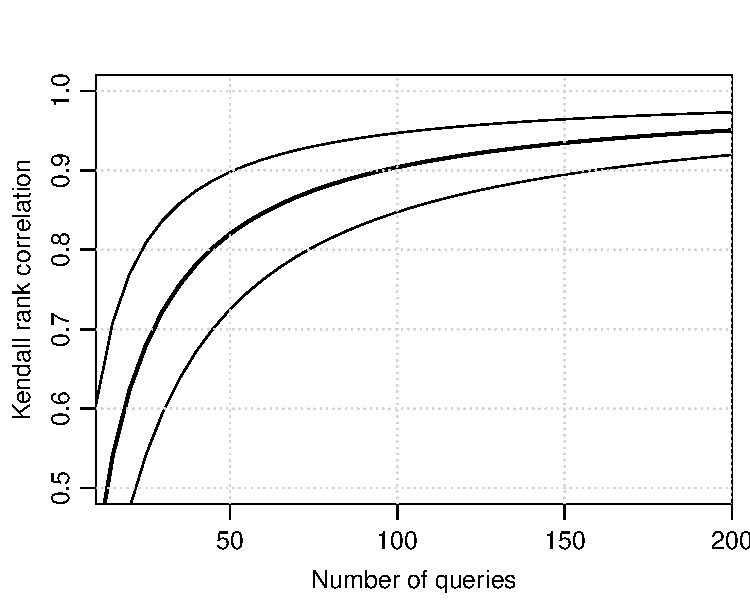
\includegraphics[scale=0.5]{plot2.pdf}%
\caption{Sample plots showing estimated $\text{E}\rho^2$ scores (left) and $\tau$ coefficients (right) as a function of the number of queries $n_q'$.}%
\label{fig:plot}%
\end{figure}

{\small\begin{verbatim}
> d.study(ah3.g, alpha = c(0.005, 0.025, 0.05))

Summary of D-Study

Call:
    queries = 50 
  stability = 0.95 
      alpha = 0.005 0.025 0.05 

Stability:
                                           Erho2                                   Phi
             -----------------------------------   -----------------------------------
       Alpha    Expected       Lower       Upper      Expected       Lower       Upper
 ----------- ----------- ----------- -----------   ----------- ----------- -----------
       0.005     0.93265     0.87737     0.96967       0.78613     0.61466      0.9023 
       0.025     0.93265     0.89311     0.96287       0.78613     0.66141     0.88039 
        0.05     0.93265     0.90062     0.95901       0.78613     0.68417     0.86796 

Required number of queries:
                                           Erho2                                   Phi
             -----------------------------------   -----------------------------------
       Alpha    Expected       Lower       Upper      Expected       Lower       Upper
 ----------- ----------- ----------- -----------   ----------- ----------- -----------
       0.005          69          30         133           259         103         596 
       0.025          69          37         114           259         130         487 
        0.05          69          41         105           259         145         439
\end{verbatim}}

The summary above shows that with 50 queries a 99\% confidence interval for $\text{E}\rho^2$ is $[0.87737, 0.96967]$, and a 90\% confidence interval on the number of queries to reach $\Phi=0.95$ is $[145, 439]$.


\section{Using the Returned Objects}

Both \texttt{g.study} and \texttt{d.study} return objects with all results from the analysis so they can be used in subsequent computations. In fact, the \texttt{ah3.g} object above contains all the G-study results, and it is provided to the \texttt{d.study} function.
The full list of available data in both objects can be obtained with the \texttt{names} function.

{\small\begin{verbatim}
> ah3.g <- g.study(ah3, drop = 0.25)
> names(ah3.g)
[1] "n.s"   "n.q"   "var.s" "var.q" "var.e" "em.s"  "em.q"  "em.e" 
> ah3.g$var.s
[1] 0.002811699

> ah3.d <- d.study(ah3.g, queries = seq(10,200,5), stability = seq(0.5,1,.05))
> names(ah3.d)
 [1] "Erho2"         "Phi"           "n.q_Erho2"     "n.q_Phi"       "Erho2.lwr"    
 [6] "Erho2.upr"     "Phi.lwr"       "Phi.upr"       "n.q_Erho2.lwr" "n.q_Erho2.upr"
[11] "n.q_Phi.lwr"   "n.q_Phi.upr"   "call"
> ah3.d$Erho2
 [1] 0.7347152 0.8059872 0.8470730 0.8737985 0.8925725 0.9064841 0.9172057 0.9257218
 [9] 0.9326493 0.9383949 0.9432373 0.9473739 0.9509485 0.9540684 0.9568151 0.9592519
[17] 0.9614284 0.9633841 0.9651511 0.9667554 0.9682185 0.9695583 0.9707896 0.9719252
[25] 0.9729758 0.9739507 0.9748576 0.9757035 0.9764944 0.9772354 0.9779311 0.9785855
[33] 0.9792022 0.9797844 0.9803349 0.9808562 0.9813506 0.9818201 0.9822666
> ah3.d$n.q_Phi.lwr
 [1]  26  32  39  48  60  77 103 146 231 487 Inf
> ah3.d$n.q_Phi.upr
 [1]   7   9  11  13  16  21  28  39  62 130 Inf
\end{verbatim}}

With all these data we can for instance plot the estimated $\text{E}\hat\rho^2$ score, with a 95\% confidence interval, as a function of the number of queries in the collection (see Figure~\ref{fig:plot}-left).

%pdf(file="M:/Papers/Information Retrieval Evaluation/055 - On the Measurement of Test Collection Reliability/plot.pdf",width=5,height=4)
%par(mar=c(3.2,3.2,2.5,0.6), mgp=c(2,0.7,0))
{\small\begin{verbatim}
> plot(ah3.d$call$queries, ah3.d$Erho2, xaxs="i", ylim=c(0.75,1), lwd=2, type="l",
+   xlab="Number of queries", ylab="Relative stability")
> lines(ah3.d$call$queries, ah3.d$Erho2.lwr) # lower confidence end
> lines(ah3.d$call$queries, ah3.d$Erho2.upr) # upper confidence end
> grid()
\end{verbatim}}


\section{Mapping G-Theory onto Data-based Indicators}

Finally, the \texttt{gt2data} function can be used to map stability indicators from Generalizability Theory onto well-known indicators such as Kendall $\tau$ correlation or sensitivity.

{\small\begin{verbatim}
> gt2data(Erho2 = 0.95, Phi = 0.8)

Estimated indicators

       Erho2         Tau       TauAP       Power Min. Confl. Maj. Confl.  Abs. Sens.
 ----------- ----------- ----------- ----------- ----------- ----------- -----------
        0.95     0.86412     0.81507      0.7826    0.010117  0.00037896   0.0097988 

         Phi  Rel. Sens.       RMSE
 ----------- ----------- -----------
         0.8     0.12389   0.0051271
\end{verbatim}}

The summary above shows that the estimated rank correlation at $\text{E}\rho^2=0.95$ is $\hat\tau=0.86412$, and that the relative sensitivity at $\Phi=0.8$ is estimated as $\hat\delta_r=12.389\%$.
In order to map the stability of a certain D-study, we can simply use the returned \texttt{d.study} object.
{\small\begin{verbatim}
> ah3.d <- d.study(ah3.g, queries = seq(10,100,10))
> gt2data(Erho2 = ah3.d$Erho2, Phi = ah3.d$Phi)

Estimated indicators

       Erho2         Tau       TauAP       Power Min. Confl. Maj. Confl.  Abs. Sens.
 ----------- ----------- ----------- ----------- ----------- ----------- -----------
     0.73472     0.41572      0.2926     0.22918     0.13072    0.030514     0.12888 
     0.84707      0.6234     0.51601     0.45241    0.056171   0.0071677    0.055058 
     0.89257     0.72355     0.63568     0.58093    0.032684   0.0028318    0.031916 
     0.91721     0.78186     0.70855     0.66165    0.021922   0.0014275    0.021348 
     0.93265     0.81993     0.75732     0.71661    0.015974  0.00082949    0.015521 
     0.94324     0.84672     0.79218     0.75633    0.012289  0.00052902    0.011919 
     0.95095     0.86658     0.81832     0.78634   0.0098238  0.00036035   0.0095132 
     0.95682     0.88188     0.83863      0.8098   0.0080808  0.00025777   0.0078147 
     0.96143     0.89405     0.85487     0.82863   0.0067955  0.00019152   0.0065638 
     0.96515     0.90394     0.86814     0.84407   0.0058161  0.00014665   0.0056117 

         Phi  Rel. Sens.       RMSE
 ----------- ----------- -----------
     0.42369     0.48914     0.16437 
      0.5952     0.30929    0.051661 
     0.68804     0.22057    0.022002 
     0.74624     0.16873    0.011186 
     0.78613     0.13514   0.0063864 
     0.81519     0.11182   0.0039579 
      0.8373    0.094779   0.0026073 
     0.85468    0.081855   0.0018006 
     0.86871    0.071753   0.0012912 
     0.88026    0.063667  0.00095472 
\end{verbatim}}

Similarly, we can use the returned \texttt{gt2data} object in subsequent computations. For instance, we can plot the estimated $\hat\tau$ correlation as a function of the query set size (see Figure~\ref{fig:plot}-right).

{\small\begin{verbatim}
> ah3.d <- d.study(ah3.g, queries = seq(10,200,5))
> ah3.i <- gt2data(Erho2 = ah3.d$Erho2)
> names(ah3.i)
[1] "tau"    "tau.ap" "power"  "minor"  "major"  "asens"  "rsens"  "rmse"   "call"  
>  plot(ah3.d$call$queries, ah3.i$tau, xaxs="i", ylim=c(0.5,1), lwd=2, type="l",
+    xlab="Number of queries", ylab="Kendall rank correlation")
>  ah3.i <- gt2data(Erho2 = ah3.d$Erho2.lwr) # lower confidence end
>  lines(ah3.d$call$queries, ah3.i$tau)
>  ah3.i <- gt2data(Erho2 = ah3.d$Erho2.upr) # upper confidence end
>  lines(ah3.d$call$queries, ah3.i$tau)
>  grid()
\end{verbatim}}

\bibliographystyle{plain}
\bibliography{gt4ireval}

\end{document}
